\section{Backlogs}

	\subsection{Les Acteurs:}
		 Les différents acteurs dans le projets sont :
		 \begin{itemize}
		 		\item L'administrateur : C'est la personne en charge de gérer le fonctionnement de l'application. 
		 		il contrôle également le calcul distribué des différents tests Selenium. Il a un rôle technique.
		 		
		 		\item L'utilisateur :  Toute personnes pouvant s'identifier sur l'application est un utilisateur.
		 		
		 		\item Un membre : C'est un utilisateur associé à un projet dans l'application.
		 		
		 		\item Un manageur : C'est un membre qui administre un projet ou plusieurs projets.
		 		
		 		\item Un client : c'est une personne extérieurs des projets de l'application, mais qui à la possibilité de 
		 											visualiser certaines parties de l'application.
		 \end{itemize}

			Les droits sont inclusif, allant de l'utilisateur à l'administrateur (utilisateur - client - membre - manageur - administrateur).

	\subsection{Backlogs}
	

\begin{center}
    \begin{tabular}{|l|p{1.5cm}|p{14cm}|}
        \hline
US01	&	\href{https://redmine-projets.smile.fr/issues/47168}{47168}	&	l'utilisateur peur s'identifier sur la page d'accueil	                                        \\
        \hline
US02	&	\href{https://redmine-projets.smile.fr/issues/47169}{47169}	&	Un utilisateur peut s'enregistrer	                                                            \\
        \hline
US03	&	\href{https://redmine-projets.smile.fr/issues/47170}{47170}	&	Un administrateur peut ajouter, modifier ou supprimer un utilisateur.	                        \\
        \hline
US04	&	\href{https://redmine-projets.smile.fr/issues/47171}{47171}	&	Un manageur peut ajouter, modifier ou supprimer un projet.	                                    \\
        \hline
US05	&	\href{https://redmine-projets.smile.fr/issues/47172}{47172}	&	Un manageur peut ajouter, modifier ou supprimer un sous-projet.	                                \\
        \hline
US06	&	\href{https://redmine-projets.smile.fr/issues/47174}{47174}	&	Un manageur peut ajouter ou supprimer un membre à son équipe.	                                \\
        \hline
US07	&	\href{https://redmine-projets.smile.fr/issues/47175}{47175}	&	Un membre peut ajouter, modifier ou supprimer un test Selenium.	                                \\
        \hline
US08	&	\href{https://redmine-projets.smile.fr/issues/47176}{47176}	&	Un membre peut lancer un test Selenium ou un projet.	                                        \\
        \hline
US09	&	\href{https://redmine-projets.smile.fr/issues/47177}{47177}	&	Un membre peut visualiser la page de détail d'un projet.	                                    \\
        \hline
US10	&	\href{https://redmine-projets.smile.fr/issues/47178}{47178}	&	Un membre peut visualiser, ajouter, modifier ou supprimer un graphique de statistique.	        \\
        \hline
US11	&	\href{https://redmine-projets.smile.fr/issues/47179}{47179}	&	Un membre peut visualiser la page de détail d'un test Selenium.	                                \\
        \hline
US12	&	\href{https://redmine-projets.smile.fr/issues/47180}{47180}	&	Un membre peut récupérer les informations d'un projet ou test via un flux RSS.	                \\
        \hline
US13	&	\href{https://redmine-projets.smile.fr/issues/47181}{47181}	&	Un membre peut exporter les informations d'un projet et tests en CSV.	                        \\
        \hline
US14	&	\href{https://redmine-projets.smile.fr/issues/47182}{47182}	&	Un membre peut exporter les informations le cahier de tests au format PDF.	                    \\
        \hline
US15	&	\href{https://redmine-projets.smile.fr/issues/47183}{47183}	&	un membre peut exporter les informations le cahier de tests au format LaTeX .	                \\
        \hline
US16	&	\href{https://redmine-projets.smile.fr/issues/47184}{47184}	&	Un membre peut exporter les informations le cahier de tests au format HTML.	                    \\
        \hline
US17	&	\href{https://redmine-projets.smile.fr/issues/47185}{47185}	&	Un administrateur peut ajouter ou supprimer des membres dans le groupe Administrateurs	        \\
        \hline
US18	&	\href{https://redmine-projets.smile.fr/issues/47186}{47186}	&	Un administrateur peut ajouter ou supprimer des membres dans le groupe Manageurs	            \\
        \hline
US19	&	\href{https://redmine-projets.smile.fr/issues/47187}{47187}	&	Un administrateur peut ajouter, modifier ou supprimer des machines pour le calcul distribué.	\\
        \hline
US20	&	\href{https://redmine-projets.smile.fr/issues/47188}{47188}	&	Un administrateur configurer les paramètres de l'application	                                \\
        \hline
US21	&	\href{https://redmine-projets.smile.fr/issues/47189}{47189}	&	Les membre ont un dashboard récapitulant l'ensemble de leurs travaux en cours.	                \\
        \hline
US22	&	\href{https://redmine-projets.smile.fr/issues/47190}{47190}	&	Le dashboard de l'administrateur	                                                            \\
        \hline
US23	&	\href{https://redmine-projets.smile.fr/issues/47191}{47191}	&	Un membre hors client peut faire des demandes à l'administrateur	                            \\
        \hline
US24	&	\href{https://redmine-projets.smile.fr/issues/47192}{47192}	&	Workflow des demandes à l'administrateur	                                                    \\
        \hline
US25	&	\href{https://redmine-projets.smile.fr/issues/47193}{47193}	&	Création d'un plugin pour interagir avec un bug tracker (Redmine,JIRA,etc...)	                \\
        \hline
US26	&	\href{https://redmine-projets.smile.fr/issues/47305}{47305}	&	Amélioration de l'identification (connexion LDAP)	                                            \\
        \hline
UST01	&	\href{https://redmine-projets.smile.fr/issues/47194}{47194}	&	Créer la liste des profiles.	                                                                \\
        \hline
UST02	&	\href{https://redmine-projets.smile.fr/issues/47195}{47195}	&	Concevoir le layout principal de l'application	                                                \\
        \hline
    \end{tabular}
\end{center}


	
\newpage{}
\subsection{User Story 01:}
L'utilisateur peut s'identifier sur la page d'accueil. La vérification se fait sur les utilisateurs en base de données
ainsi que ceux présent dans le LDAP.


\begin{center}
      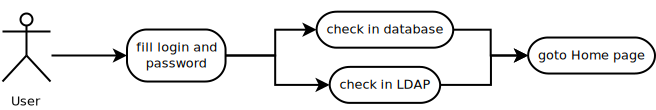
\includegraphics[width=0.7\textwidth]{US01}
\end{center}



\begin{center}
      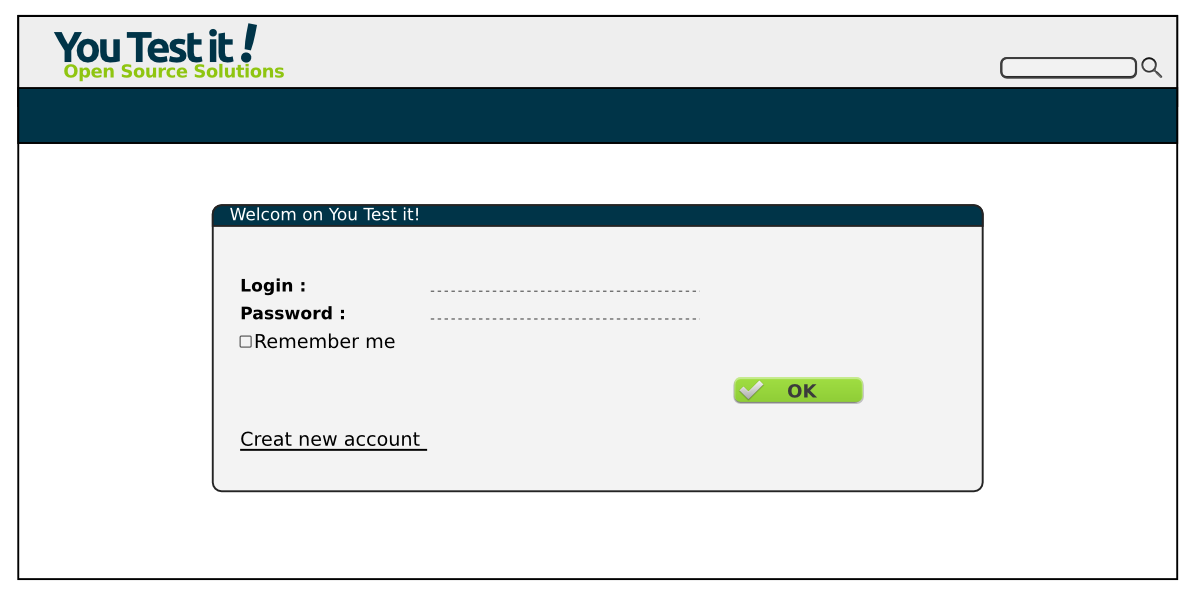
\includegraphics[width=0.9\textwidth]{interface-US01-login}
\end{center}



% \newpage
\subsection{User Story 02:}
Un utilisateur peut s'enregistrer. Un administrateur doit en suite valider l'inscription et associer un rôle à l'utilisateur.

\begin{figure}[!h]
  \begin{center}
        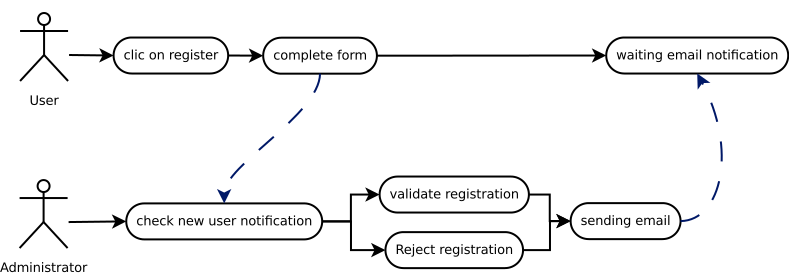
\includegraphics[width=0.7\textwidth]{US02}
        \label{US02-dia}
  \end{center}
\end{figure}

\newpage
\subsection{User Story 03:}
Un administrateur peut ajouter, modifier ou supprimer un utilisateur.

\begin{figure}[!h]
  \begin{center}
        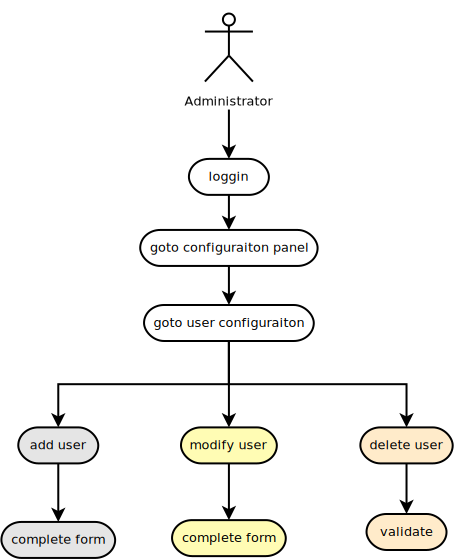
\includegraphics[width=0.5\textwidth]{US03}
        \label{US03-dia}
  \end{center}
\end{figure}

\newpage{}
\subsection{User Story 04:}
Un manageur peut ajouter, modifier ou supprimer un projet.

  \begin{center}
        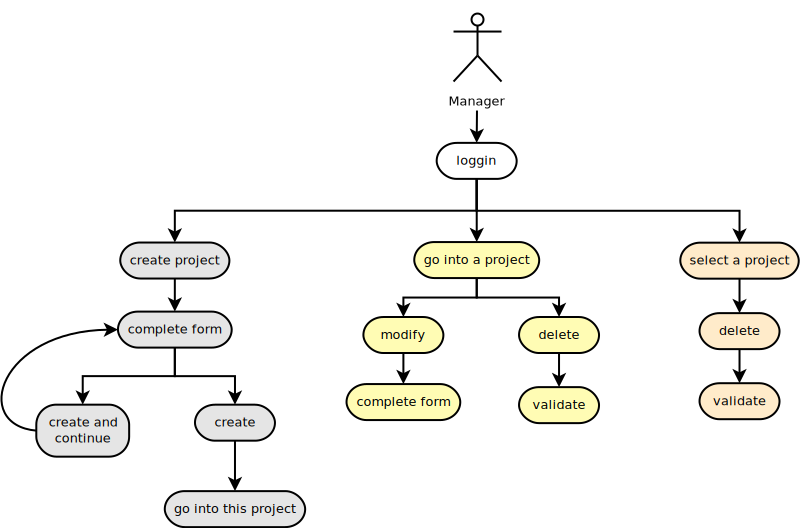
\includegraphics[width=0.7\textwidth]{US04}
  \end{center}


\newpage{}
  \begin{center}
        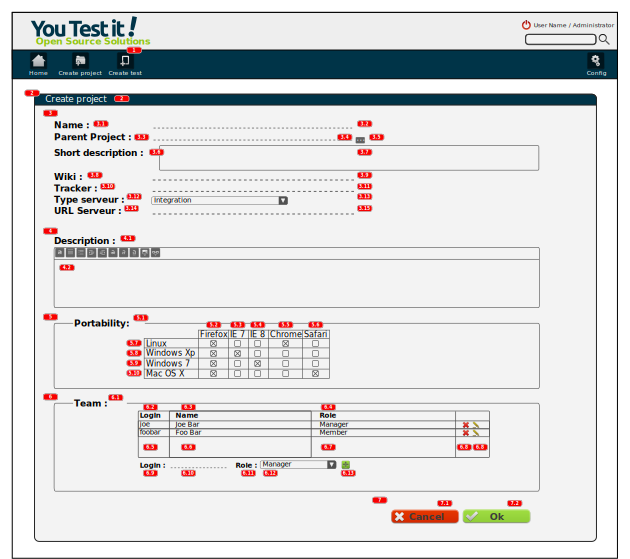
\includegraphics[width=0.8\textwidth]{interface-US04-create-project}
  \end{center}

\newpage
\subsection{User Story 05:}
Un manageur peut ajouter, modifier ou supprimer un sous-projet.


\begin{figure}[!h]
  \begin{center}
        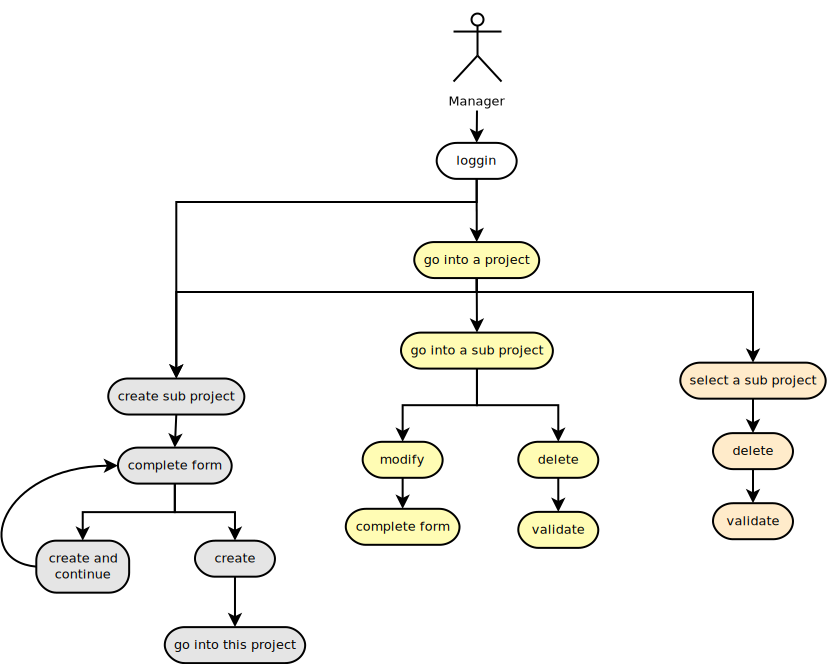
\includegraphics[width=0.7\textwidth]{US05}
        \label{US05-dia}
  \end{center}
\end{figure}

\newpage
\subsection{User Story 06:}
Un manageur peut ajouter ou supprimer un membre à son équipe.


\begin{figure}[!h]
  \begin{center}
        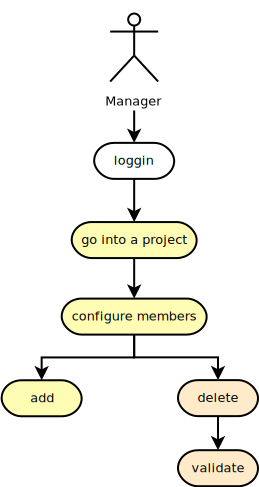
\includegraphics[width=0.3\textwidth]{US06}
        \label{US06-dia}
  \end{center}
\end{figure}

\newpage{}
\subsection{User Story 07:}
un membre peut ajouter, modifier ou supprimer un test Selenium. La suppression est soumise à la validation
du manager.


  \begin{center}
        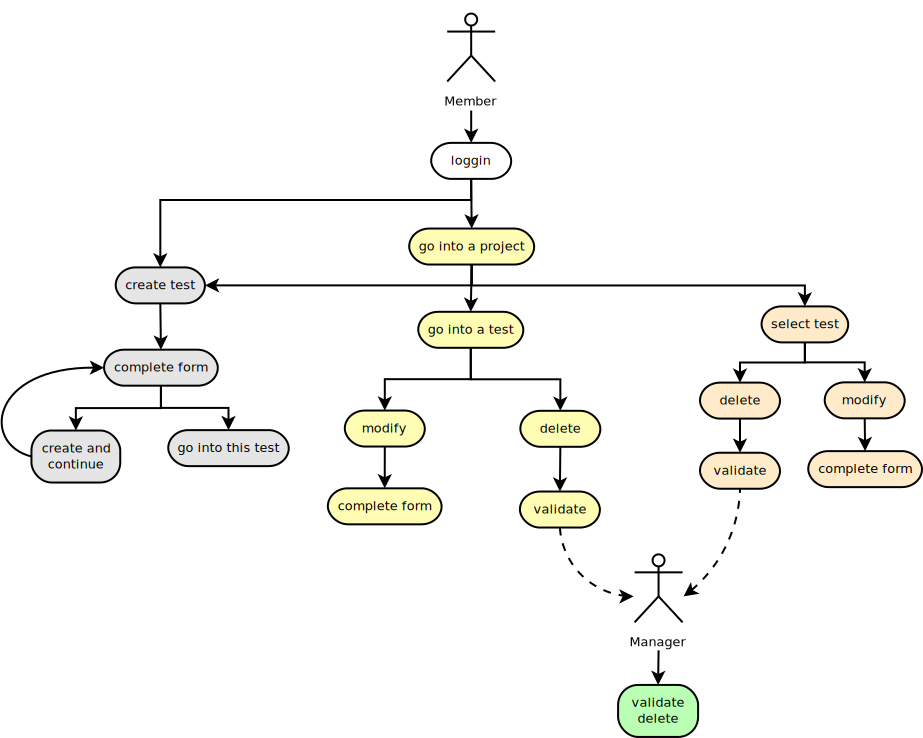
\includegraphics[width=0.8\textwidth]{US07}
  \end{center}

\newpage{}
  \begin{center}
        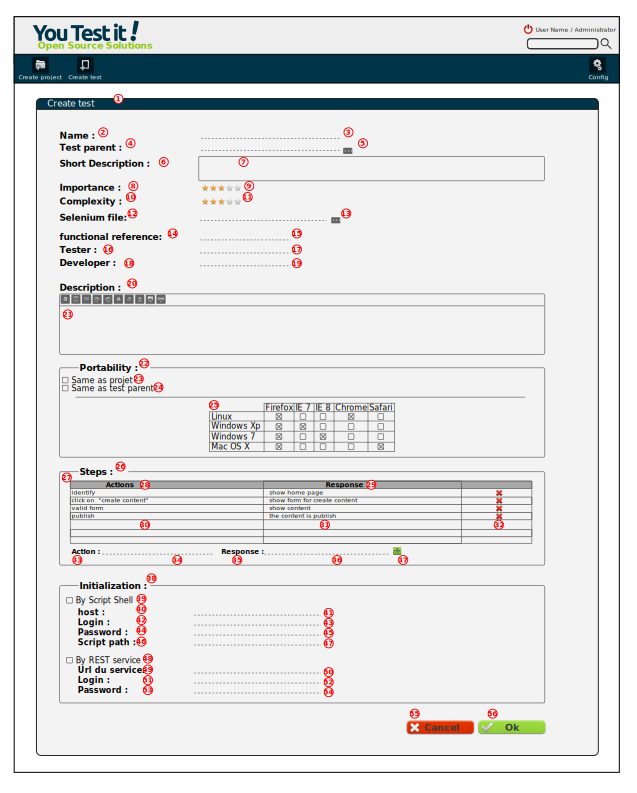
\includegraphics[width=0.9\textwidth]{interface-US07-create-test}
  \end{center}

\newpage
\subsection{User Story 08:}
Un membre peut lancer un test Selenium ou un projet.


\begin{figure}[!h]
  \begin{center}
        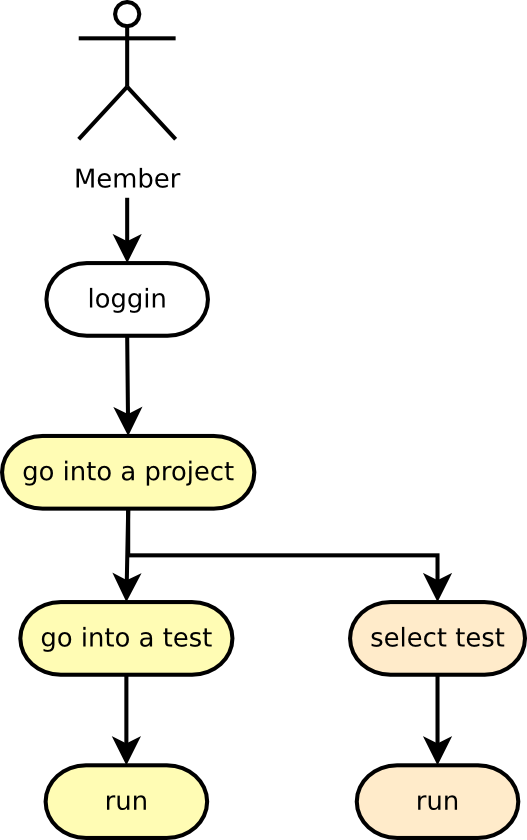
\includegraphics[width=0.25\textwidth]{US08}
        \label{US08-dia}
  \end{center}
\end{figure}

\newpage{}
\subsection{User Story 09:}
Un membre peut visualiser la page de détail d'un projet.

  \begin{center}
        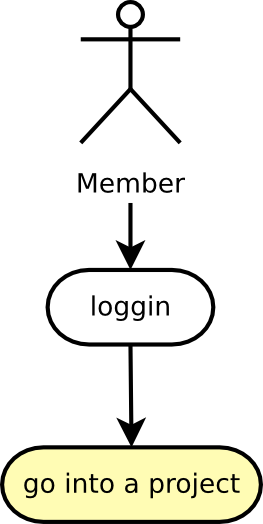
\includegraphics[width=0.1\textwidth]{US09}
  \end{center}

  \begin{center}
        \includegraphics[width=0.9\textwidth]{interface-US09-project-home}
  \end{center}

\newpage{}
\subsection{User Story 10:}
Un membre peut  visualiser, ajouter, modifier ou supprimer un graphique de statistique.


  \begin{center}
        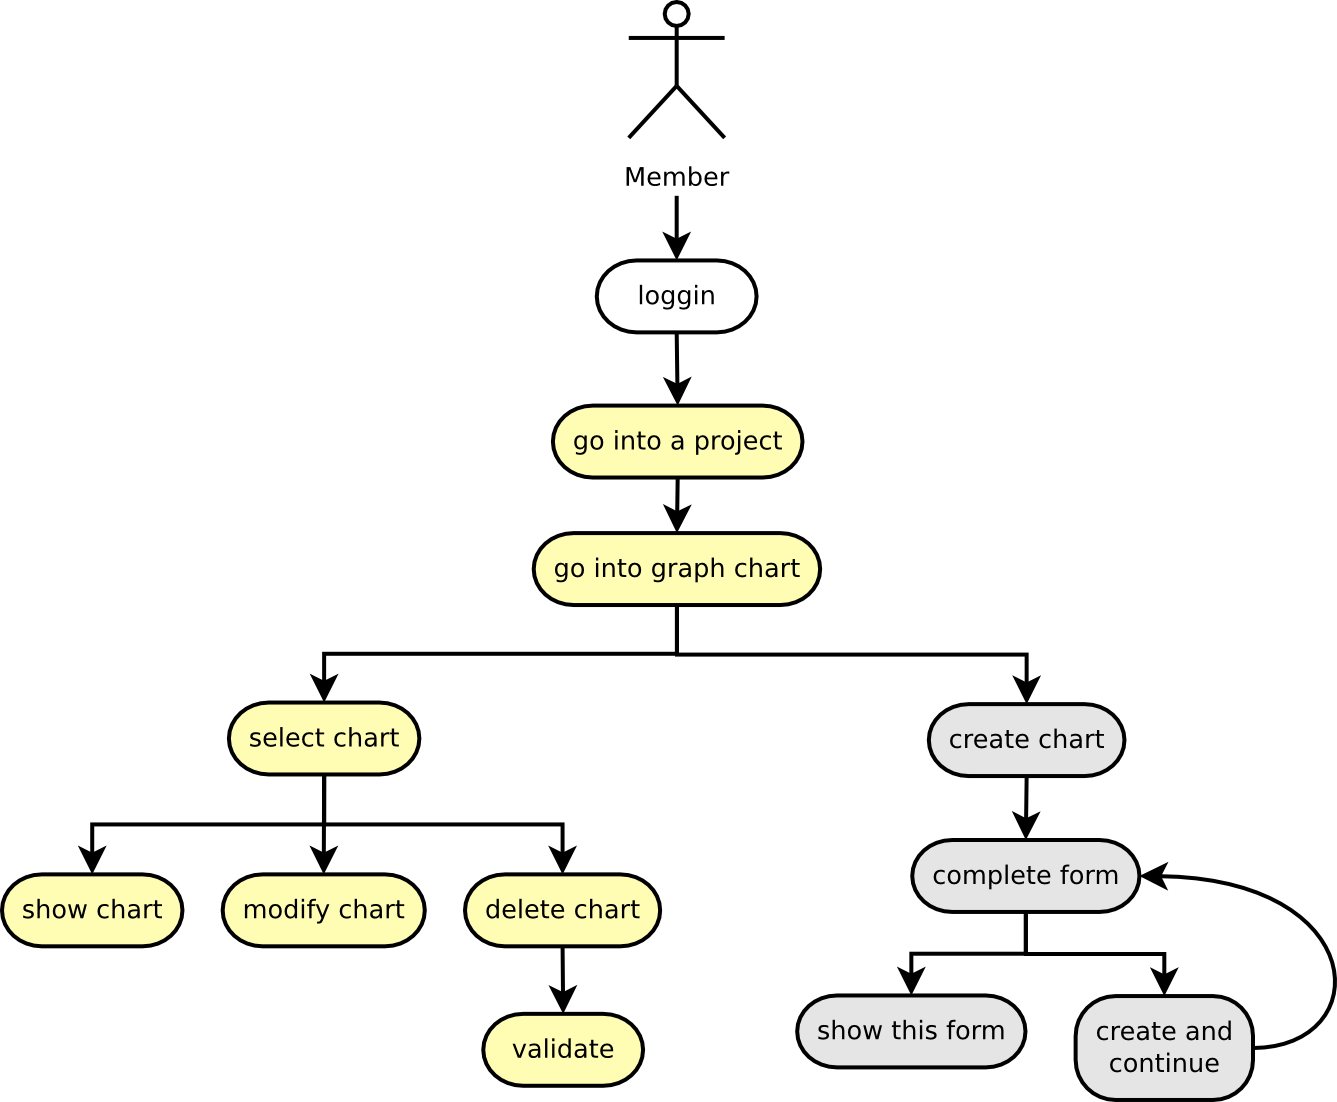
\includegraphics[width=0.65\textwidth]{US10}
  \end{center}


\newpage{}
\subsection{User Story 11:}
Un membre peut visualiser la page de détail d'un test Selenium.

  \begin{center}
        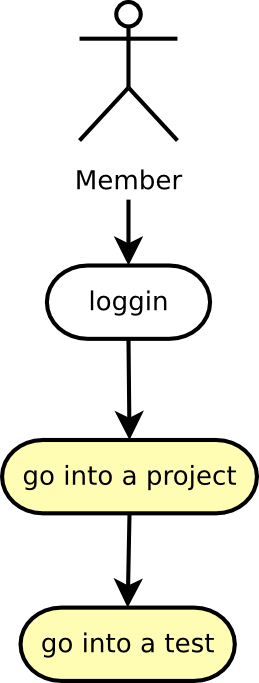
\includegraphics[width=0.1\textwidth]{US11}
  \end{center}

  \newpage{}
  \begin{center}
        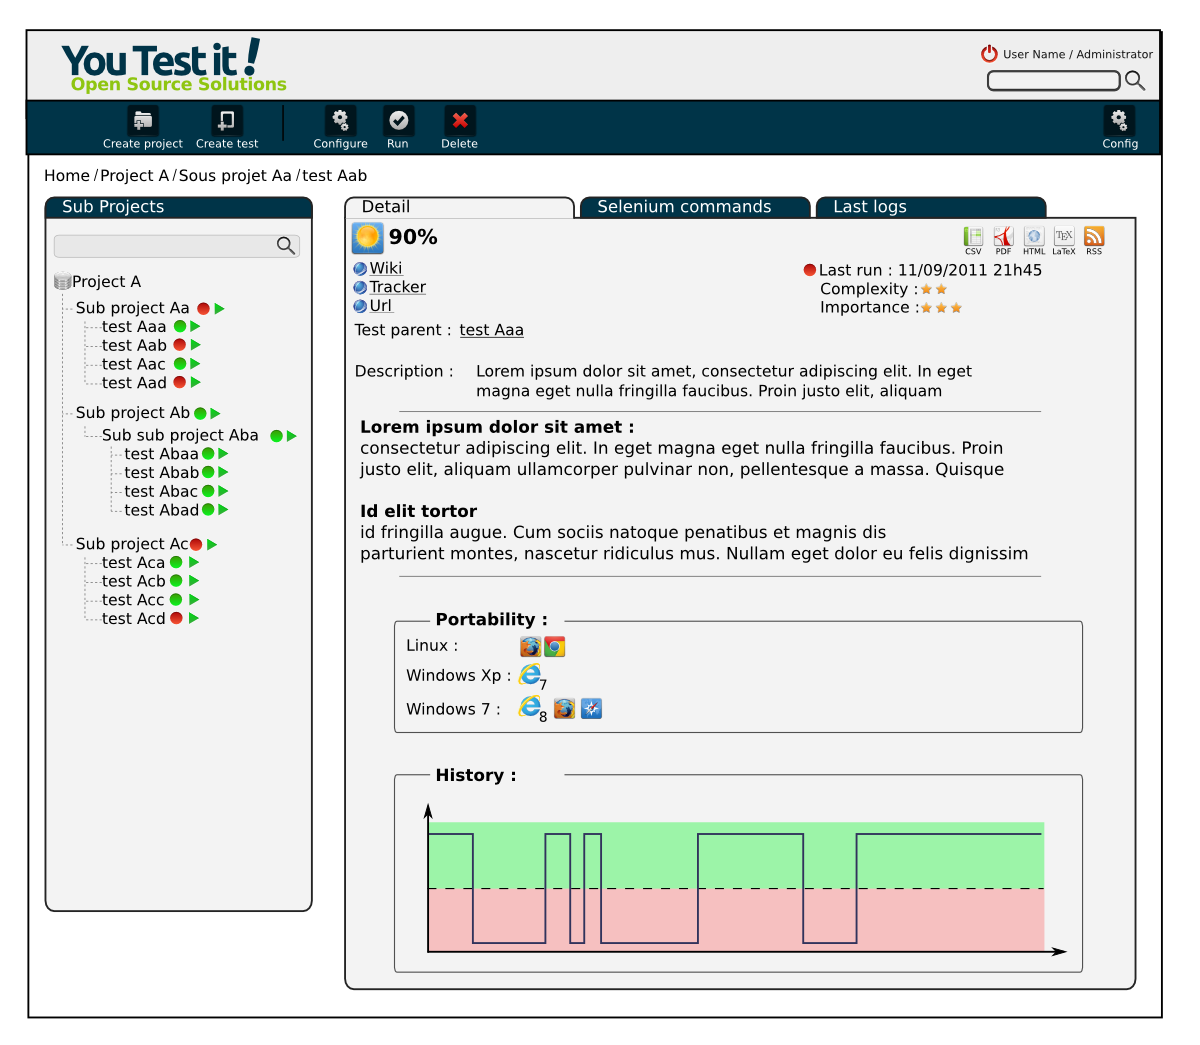
\includegraphics[width=0.9\textwidth]{interface-US11-test-home}
  \end{center}


\subsection{User Story 12:}
Un membre peut récupérer les informations d'un projet ou test via un flux RSS.

\begin{figure}[!h]
  \begin{center}
        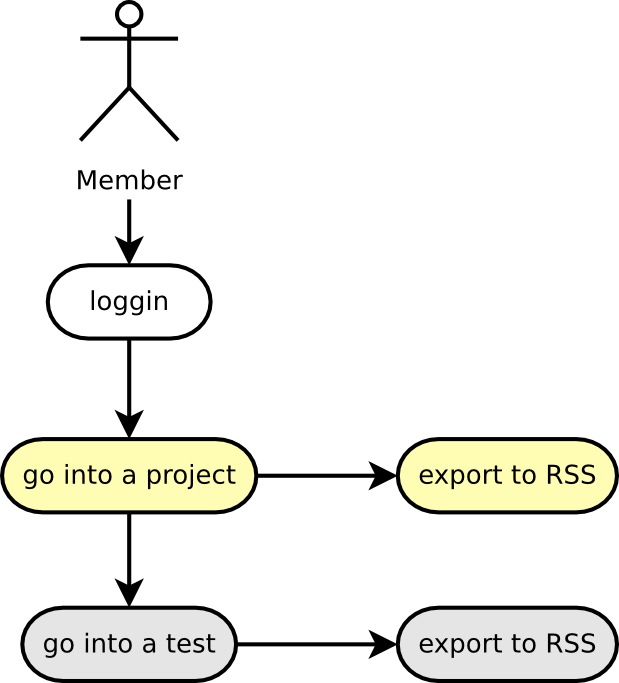
\includegraphics[width=0.3\textwidth]{US12}
        \label{US12-dia}
  \end{center}
\end{figure}

\newpage{}
\subsection{User Story 13:}
un membre peut exporter les informations d'un projet et tests en CSV.

  \begin{center}
        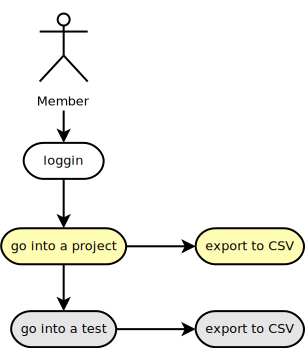
\includegraphics[width=0.3\textwidth]{US13}
  \end{center}


\subsection{User Story 14:}
un membre peut exporter les informations le cahier de tests au format PDF.


\begin{figure}[!h]
  \begin{center}
        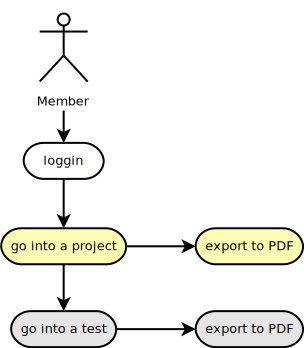
\includegraphics[width=0.3\textwidth]{US14}
        \label{US14-dia}
  \end{center}
\end{figure}

\newpage{}
\subsection{User Story 15:}
Un membre peut exporter les informations et le cahier de tests d'un projet au format \LaTeX{}.


  \begin{center}
        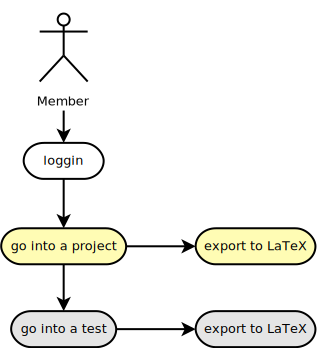
\includegraphics[width=0.3\textwidth]{US15}
  \end{center}

\newpage{}
\subsection{User Story 16:}
un membre peut exporter les informations le cahier de tests au format HTML.


  \begin{center}
        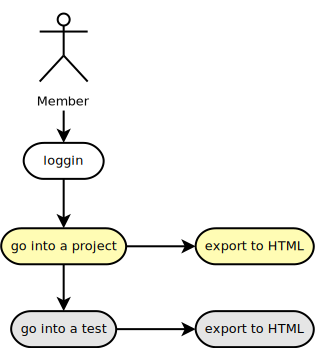
\includegraphics[width=0.3\textwidth]{US16}
  \end{center}

\newpage
\subsection{User Story 17:}
Un administrateur peut ajouter ou supprimer des membres dans le groupe Administrateurs


\begin{figure}[!h]
  \begin{center}
        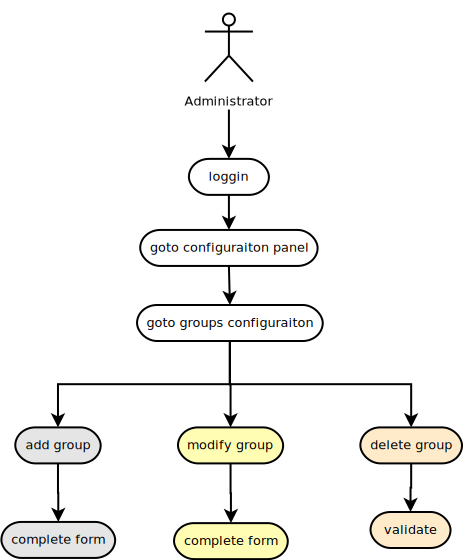
\includegraphics[width=0.5\textwidth]{US17}
        \label{US17-dia}
  \end{center}
\end{figure}

\newpage{}
\subsection{User Story 18:}
Un administrateur peut ajouter ou supprimer des membres dans le groupe Manageurs.


  \begin{center}
        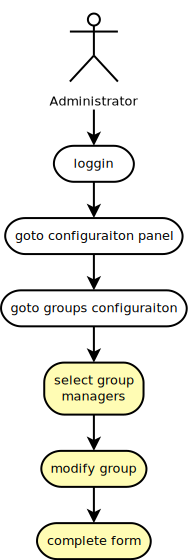
\includegraphics[width=0.25\textwidth]{US18}
  \end{center}

\newpage{}
\subsection{User Story 19:}
Un administrateur peut ajouter, modifier ou supprimer des machines pour le calcul distribué.


  \begin{center}
        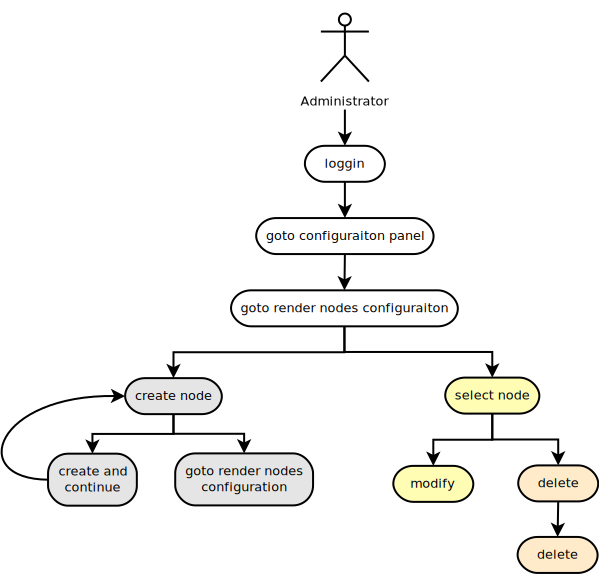
\includegraphics[width=0.6\textwidth]{US19}
  \end{center}

\newpage
\subsection{User Story 20:}
Un administrateur configurer les paramètres de l'application (adresse mail, nombre de calcul simultané, etc...)


\begin{figure}[!h]
  \begin{center}
        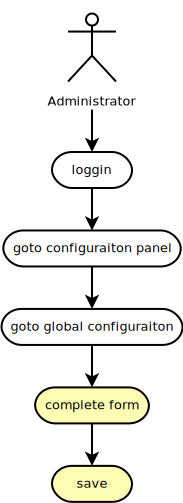
\includegraphics[width=0.25\textwidth]{US20}
        \label{US20-dia}
  \end{center}
\end{figure}

\newpage{}
\subsection{User Story 21:}
Les membres ont un dashboard récapitulant l'ensemble de leurs travaux en cours.	


  \begin{center}
        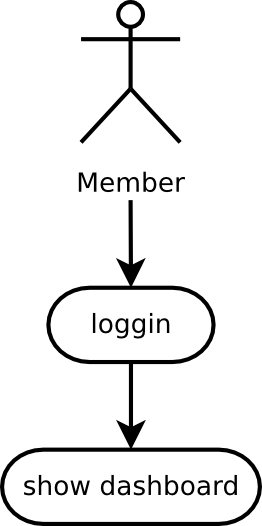
\includegraphics[width=0.25\textwidth]{US21}
  \end{center}

\newpage{}
\subsection{User Story 22:}
Le dashboard de l'administrateur contient des blocs supplémentaires, comme pour la disponibilité des machines,
ou les demandes qui lui sont adressées.


  \begin{center}
        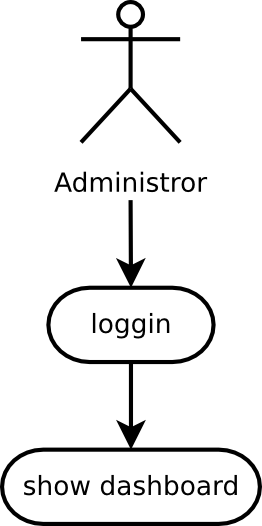
\includegraphics[width=0.2\textwidth]{US22}
  \end{center}

\newpage
\subsection{User Story 23:}
Un membre hors client peut faire des demandes à l'administrateur:

\begin{itemize}
  \item demande d'ajout de plugins
  \item demande d'ajout de machine spécifique
  \item etc...
\end{itemize}



\begin{figure}[!h]
  \begin{center}
        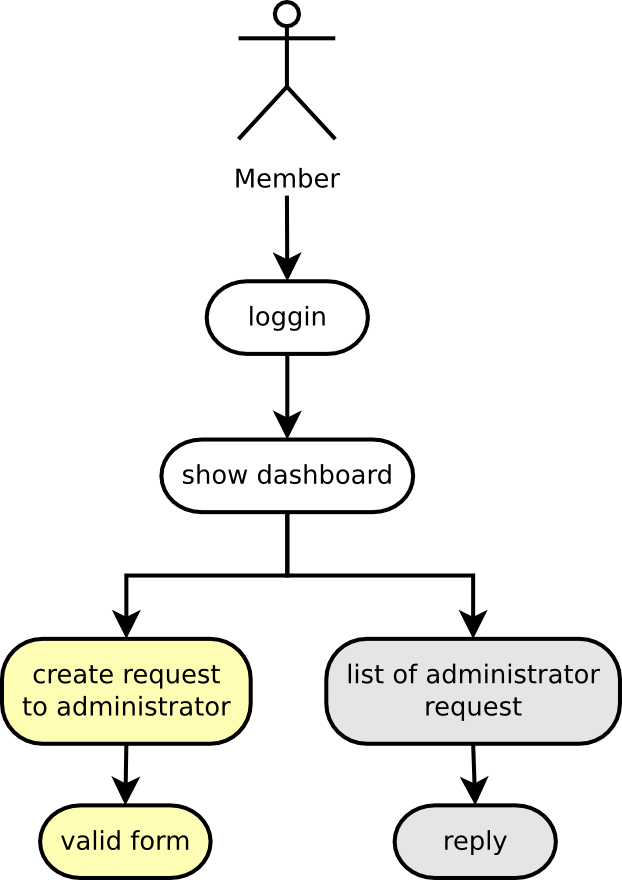
\includegraphics[width=0.5\textwidth]{US23}
        \label{US23-dia}
  \end{center}
\end{figure}

\newpage
\subsection{User Story 24:}
Workflow des demandes à l'administrateur.  Le workflow de l'administrateur doit être relativement
simple. Il se base sur quelque états :

\begin{itemize}
  \item pris en compte
  \item traité
  \item traité, disponible après redémarrage de l'application
  \item complément d'information
  \item rejeté
  \item clos
\end{itemize}


\begin{figure}[!h]
  \begin{center}
        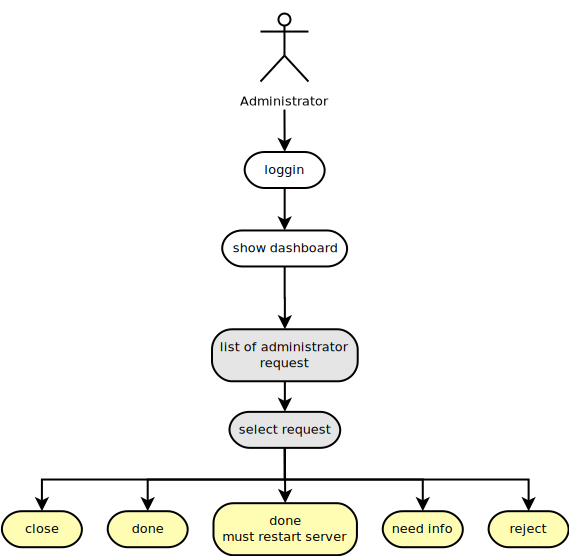
\includegraphics[width=0.7\textwidth]{US24}
        \label{US24-dia}
  \end{center}
\end{figure}

\newpage{}
\subsection{User Story 25:}
Création d'un plugin pour interagir avec un bug tracker (Redmine,JIRA,etc...)


  \begin{center}
        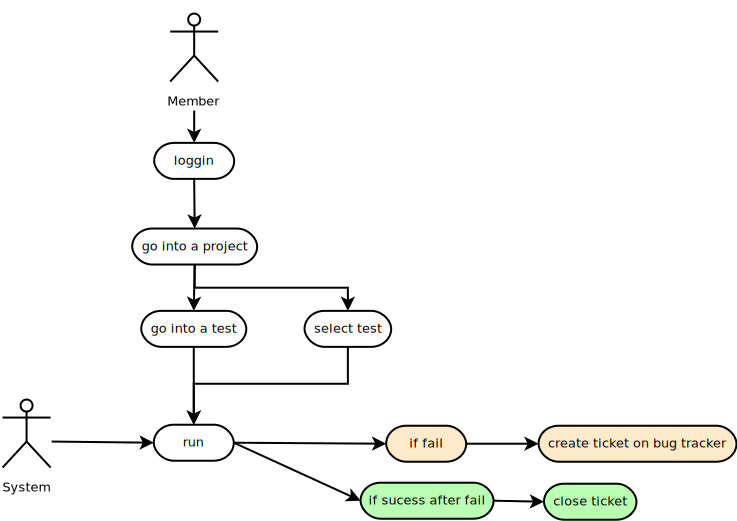
\includegraphics[width=0.7\textwidth]{US25}
  \end{center}

\newpage{}
\subsection{User Story 26:}
Amélioration  de l'identification et des services liés aux utilisateurs


  \begin{center}
        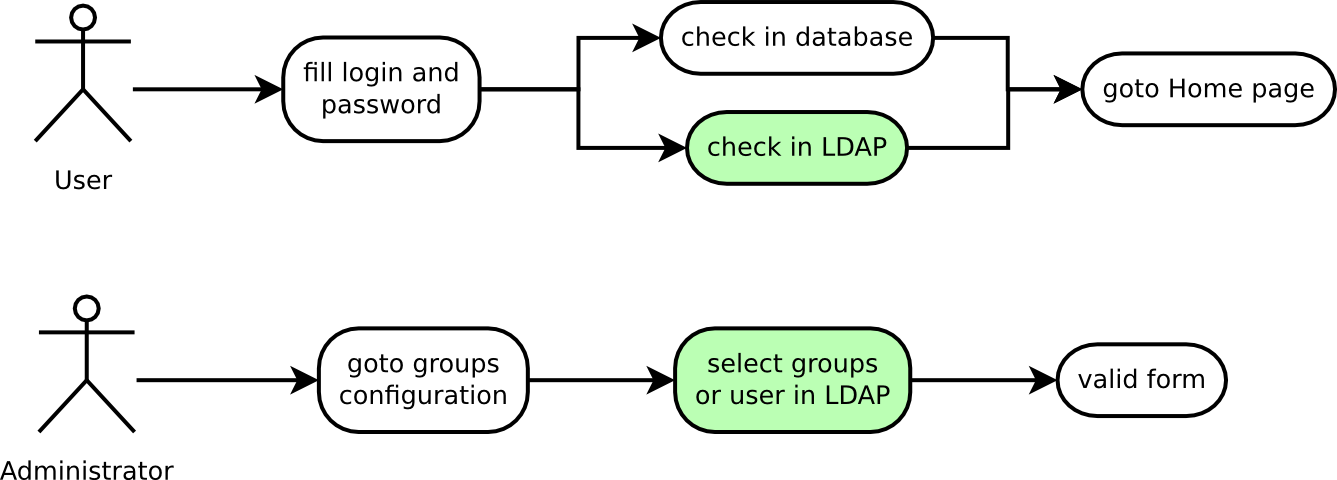
\includegraphics[width=0.7\textwidth]{US26}
  \end{center}



\subsection{Technical User Story 01:}
Créer la liste des profiles.

\subsection{Technical User Story 02:}
Concevoir le layout principal de l'application



	
